\documentclass[11pt,letter]{article}
\usepackage[top=0.70in, bottom=0.7in, left=1.1in, right=1.1in]{geometry}
\usepackage{graphicx} % Required for inserting images
\usepackage{xcolor} 
\definecolor{Accent}{HTML}{bd2b00} 
\usepackage[numbers,compress,super]{natbib}
\usepackage{gensymb}
\usepackage{hyperref}
\hypersetup{colorlinks,citecolor = Accent, linkcolor = Accent,urlcolor = Accent, breaklinks=true}
\usepackage{cleveref}
\usepackage[labelfont=bf]{caption}
\bibliographystyle{unsrtnat}

\RequirePackage[labelfont={bf,sf},%
                font={small, sf}]{caption}

\usepackage{lineno}
\renewcommand\linenumberfont{\normalfont\tiny\color{gray}}

\begin{document}

\title{Overlooked model uncertainties may misinform forest management strategies
% Alternative title: Integrating full model uncertainties could improve forest management
}

\author{Victor, Jérôme, Isabelle} % and more?
\date{}
\maketitle 
%emw19May -- overall this seems much better! The text is still not as tight as I would hope for a short format journal though. 

\noindent\rule{\textwidth}{0.3pt}
%emw19May -- One thing that is tricky here is the link the management. I think it's fine (and even good!) but it makes the number of links you need to make for the reader to get to your point longer. (For example, in your abstract you could just say 'Forests play a major role in mitigating climate change and maintaining that requires robust forecasts of their future composition ...' but the management connection takes more steps). Just being aware of this could help you make it as easy as possible on the reader. 
%emw19May --  alternative abstract text: 
Forests play a major role in mitigating climate change, but they must be carefully managed to maintain this role through increasing anthropogenic threats. Robust management requires robust forecasts, but current projections are the outcome of layered models and highly variable. Identifying the drivers of this variability---whether it is from different emissions scenarios, uncertainty in climate models or ecological models---is thus critical to advancing management. To address this, we compare over 1350 ecological models and climate scenarios in forecasts for forests across Europe. Our approach considers a gradient of more mechanistic (`process-based') to correlative models of species distributions. We find that difference between ecological models represent the largest source of uncertainty (40 to 64\%), surpassing both climate models and vastly different climate scenarios (e.g., SSP2 vs. SSP5). We also find areas with relatively consistent projections where management could take immediate action. Our results point to current limitations in ecological forecasting methods that make management difficult. At the same time they provide a framework to identify regions with the most consistent projections and those regions where high ecological uncertainty, which may benefit from diversified and more risk-adverse strategies until ecological forecasting advances.

% \textbf{Abstract---still need work:} Forests play a major role in mitigating climate change, but increasing threats to forests from climate change have heightened the importance of managing these systems. Robust forecasts of forest composition with increasing climate change are critical to this aim, but are currently highly variable. To help guide management in the face of this variability and understand where we can most rapidly reduce uncertainty through improved models, we compare over 1350 ecological models and climate scenarios in forecasts for forests across Europe. Our approach considers a gradient of more mechanistic (`process-based') to correlative models of species distributions and find that difference between ecological models represent the largest source of uncertainty (40 to 64\%), surpassing both climate models and vastly different climate scenarios (e.g., SSP2 vs. SSP5). We also find areas with relatively consistent projections [give overview of these and say that this could reduce uncertainty in how to manage for these areas]. Our results point to current limitations in ecological forecasting methods, identifies avenues to lower uncertainty % vvdm: too vague?
% and, suggests that managers need to internalize ecological uncertainty through diversified and more risk-adverse strategies.

\noindent\rule{\textwidth}{0.3pt}

\linenumbers

\subsection*{Main}
%
%Intro:
%1. Basically first two paragraphs you have combined (we need forests to
%store C, and they are doing poorly) ending on the need for better
%guidance of forest management
%2. This is hard because we have a lot of biological models and they give
%different answers, and for management we need to layer on the future
%climate models ...
%- Go into briefly the correlative versus process models -- they
%differ  but we're not sure which is best
%- Given we don't have one great approach to build to (and we have
%run out of time), so maybe we move on and accept the diversity
%- Transition to something explaining the layers of models we need
%to consider to capture climate to biology
%3. Back to what we need to do with the models for forest management
%- Here you might touch on what we could do with this, get in some
%of the stuff I highlighted in the discussion that you need to foreshadow
%for readers.


%From J Chave:
%Climate change has direct impact on a myriad of ecosystem processes, and forests are especially vulnerable. European temperatures are rising twice as fast as the global average (Copernicus Climate Change Service, 2024), and unprecedented pulses of tree mortality have benn reported in the last decade, across the range of forest species (Senf et al, 2020). As a consequence, some European forests are now net CO2 sources (Hadden and Grelle, 2016; Karelin et al, 2021), due to decreased growth (Hadden and Grelle, 2016; van der Woude et al, 2023), increased burned areas (Carnicer et al, 2022; Kelly et al, 2024), and increased pest or drought-related dieback driven (Cienciala and Melichar, 2024; Karelin et al, 2021; Latifovic and Arain, 2024).  Implementation strategies are rolled out in spite of the uncertainty of the scenarios.

%1. Basically first two paragraphs you have combined (we need forests to
%store C, and they are doing poorly) ending on the need for better
%guidance of forest management
% the baby: with climate change, we need to safeguard and adapt forests, as they play a major role in mitigating its effects
Forests are key to climate change mitigation policies and achieving carbon neutrality  \citep{Korosuo2023, Hyyrynen2023}. Yet, forests are increasingly under pressure. In Europe, temperatures are rising twice as fast as the global average \citep{CCCS2024}, and unprecedented pulses of tree mortality  have been reported in the last decade \citep{Senf2020}. As a result, some European forests are becoming net CO$_2$ sources \citep{Hadden2016, Karelin2021}, due to decreased growth \citep{Hadden2016, Woude2023}, larger burned areas \citep{Carnicer2022, Kelly2024}, and increased pest- and drought-induced dieback \citep{Karelin2021, Cienciala2024, Latifovic2024}. 

Forest managers working to minimize current threats while also promoting long-term adaptation to climate change rely on forecasts of shifts in critical tree species. Species shifts are predicted to have major impacts on timber production and on the forest economic sector \citep{Wessely2024, Hanewinkel2013}. To preserve the socio-economic functions of forests, managers need to know whether the current species will be able to tolerate future climate conditions, whether they can rely on natural regeneration, or whether they should consider new species opportunities. To date, however, ecological models have struggled to provide practical insights for forest management.

 % In this context of high uncertainty, better guidance  is needed to implement successful strategies.
% and evidence-based projections are

%2. This is hard because we have a lot of biological models and they give
%different answers, and for management we need to layer on the future
%climate models ...
%- Go into briefly the correlative versus process models -- they
%differ  but we're not sure which is best
%- Given we don't have one great approach to build to (and we have
%run out of time), so maybe we move on and accept the diversity
%- Transition to something explaining the layers of models we need
% the werewolf: We have many models, we don't know which one is the best. Most decisions rely on limited models without much insight into what drives differences in projections. This can mask significant uncertainties and ultimately threaten the success of forest management decisions
% the silver bullet: accept a greater diversity of models (scientific approaches, hypothesis), and figure out how to safeguard forests by gaining a better understanding of uncertainties, i.e., merging across biological and climatological components (uncertainty budget framework)
Different models, ranging from correlative to more mechanistic approaches, often provide highly divergent projections \citep{Morin2009, Keenan2011a, Cheaib2012, Takolander2019}. While it remains unclear under which conditions one approach is more reliable than another \citep{VanderMeersch2024}, most projections still rely on a limited set of models \citep{Dyderski2018, Wessely2024, Hanewinkel2013, Schueler2014}, masking significant uncertainties and ultimately increasing the risk of policy and management failures \citep{Dawson2011}. 
% below: important but wordy, rephrase
% We often lack a comprehensive understanding of what drives differences between projections and a robust estimation of uncertainty \citep{Simmonds2024}. 

%3. Back to what we need to do with the models for forest management
%- Here you might touch on what we could do with this, get in some
%of the stuff I highlighted in the discussion that you need to foreshadow
%for readers.

%emw19May --  I love this sentence, but it feels too similar to the next one (and will readers understand the link between 'policy relevant opportunities' and forest management? Not sure but either sentence could work I think as long as you link these fore readers. 
% Gaining a better understanding of where uncertainties originate and how they relate is a first step to identify opportunities  to address policy-relevant questions \citep{Urban2016, Saltelli2020, Johnson2024, Simmonds2024}. 

% New paragraph here!
% "For forest managers to do this given our current reality of uncertain forecast, they need better info...
% high uncertainty brought about by climate change
To incorporate the current reality of uncertain forecasts, forest managers require better information on the processes that cause uncertainty. %emw19May -- I think here you need to move up some of what you have below -- spell out that current models have layers to them ('that can account for all the components of ')
Current projections have several layers of climatological and biological uncertainties, including socioeconomic scenarios, global climate models, ecological models, down to the species level. If the main driver of variation across projections is the differences between ecological models, even more than different global emissions scenarios, it becomes critical to encompass a wide range of models. Failing to do so could lead to overly confident predictions about which species will or will not be able to survive in future climates, ultimately leading to counterproductive or even detrimental forest management decisions.
Consistency between projections can also reveal regions where models agree and where uncertainty is lower.
%Given the urgency of climate change, 
%emw19May -- I would cut the below sentence and see if you can get by without it. 
% We must incorporate the diversity of models and merge across ecological and climatological models to provide a complete picture of both the threats and opportunities for forests. 

%emw19May -- below, consider integrating methods more? Something like ... (you could also add 'hybrid' term here):

To this aim, we combined over 1350 projections from models of future forest tree species distributions (from 1970 to 2100, at a 0.1\degree~spatial resolution). We incorporated a wide range of ecological models, from more mechanistic (‘process-based’) to correlative models to `hybrid' models. To forecast from these models we also considered climate model variability (5 global climate models with different climate sensitivities) and two emissions (`forcing') scenarios, resulting in 10 different future climate simulations. Our dataset included 9 tree species, both deciduous and coniferous, adapted to diverse climatic conditions across Europe.

Including variability from the ecological, climatological and emissions scenarios allowed us to quantify the contribution of each component to the total variation across projections. This approach represents a significant advancement over previous studies, which overlooked large portions of uncertainty. Such advances could lead to more informed decision-making to improve the resilience of forests. 



% Note: what should be in the intro:
% huge differences between projections, more importanmt than species or SSP, toget a comprehensive assesment of the magnitude of climatic change?
%  ignoring a large portion of uncertainty in psecies range projections due to modelling approaches can thus lead to baaad decisions.


\begin{figure}
	\centering
	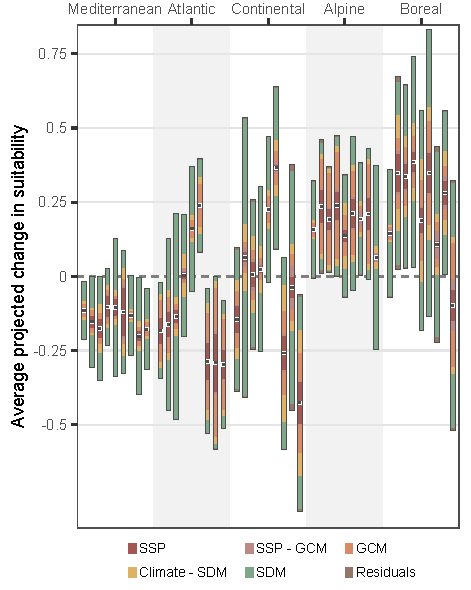
\includegraphics[width=1\linewidth]{figures/anova_within_species_byecoregion-1.pdf}
	\caption{\textbf{Ecological models represent the main source of uncertainty in future projections of species climatic suitability across European biomes (2080-2100).} This figure illustrates the level of uncertainty associated with projected changes in suitability relative to the historical period (1970–2000), \textbf{(a)} for each species within biome and \textbf{(b)} across all species and biomes. We distinguish 5 main uncertainty sources: (i) the future scenario (SSP), (ii) the climate model used to generate the climate projections (GCM), (iii) the interactions between the SPP and the GCM, (iv) the species distribution modeling method (SDM), and (v) the interactions between SDM and climate projections (both GCMs and SSPs). For each species, the black line represents the mean projection, across all GCMs, SSPs, and SDMs. 90\% uncertainty ranges were calculated additively and symmetrically around the mean.}
	\label{fig:anovaspecies}  %emw19May -- what is (c)? Add to caption.
\end{figure}

\subsection*{Results and discussion}

% Our dataset included 9 tree species, both deciduous and coniferous, adapted to diverse climatic conditions across Europe. We simulated their suitability from 1970 to 2100, at a 0.1\degree~spatial resolution, using a range of ecological models a range of hypotheses and a range of calibration methods. We used  2 forcing scenarios and 5 global climate models with different climate sensitivities resulting in 10 different future climate simulations.

% Overall we found that the choice of the ecological forescast model explained 51% of the variation across species and biomes, while uncertainty in the socio-economic pathway explained only 35% of the variation (Figure 1). The current driest biome, the Mediterranean region, showed a consistent decline in suitability across all species, but a great uncertainty due to differences in ecological forescast models. The Atlantic and Continental biomes displayed contrasted results depending on the species, with reduced suitability for the Northern species (Scots pine, Silver fir) and increaded suitability for Southern species (pubescent oak and evergreen oak). Few of the detected trends were significant, however, due to the large total uncertainty. Likewise, in Alpine biomes, all trends were towards increased suitability but barely significant ... 

% uncertainty in ecological models can drive more variation than vastly different climate scenarios 
%emw19May -- I would write this past tense but up to you ...
Differences between ecological models consistently explained more variation than vastly different climate trajectories. Overall, we found that the choice of the ecological model explained 51\% of the variation across species and biomes, while uncertainty in the socio-economic pathway explained only 35\% of the variations (\Cref{fig:anovaspecies}). The current driest biome, the Mediterranean region, showed a consistent decline in suitability across all species. The Atlantic and Continental biomes displayed contrasting results depending on the species. 
%emw19May -- any way to edit below sentence so it explains the biology/policy/management more than the stats? Maybe: The total uncertainty, however, makes few of these detected trends easy to act on (few were significant, see ANOVA). 
Few of the detected trends were significant, however, due to the large total uncertainty (\Cref{fig:anovaspecies}). One striking example is the climatic suitability change of sessile oak in the Atlantic region, where this species represents an important cultural and economic value, and for which more than 80\% of the uncertainty in climate change impact projections was due to variations among ecological models. 

% The differences among climate model projections (GCMs) and socioeconomic scenarios (SSPs). 
% in the Continental ecoregion, differences across models account for 73.7% of the total uncertainty of beech future suitability, despite being within the core of its present distribution. Similarly, SDM is the main source of uncertainty for sessile and pedunculate oaks (respectively 57% and 76.8%, Figure 22).

%emw19May -- consider a subheader? Also you have a couple places where you give the topic sentence at the start and again at the end of the paragraph and I am not sure it works, so I edited it. 
Subheader: Mechanistic to correlative models contribute to high uncertainty ... 

Accounting for more diverse ecological models led to a more comprehensive range of potential future change in suitability (\Cref{fig:cascade}), revealing the high divergence between ecological models and the persistent gaps in our understanding of species responses to climate change. Considering only correlative models would have misled to an overestimation of the contribution of climate projections (forcing scenarios, climate models, and their two-way interaction) to the total projection uncertainty in all regions, except the Mediterranean. In particular, divergence between climate models would have appeared to contribute as much as ecological models to projection uncertainty (on average, 36.6\% and 37.5\%, respectively). 



\begin{figure}
	\centering
	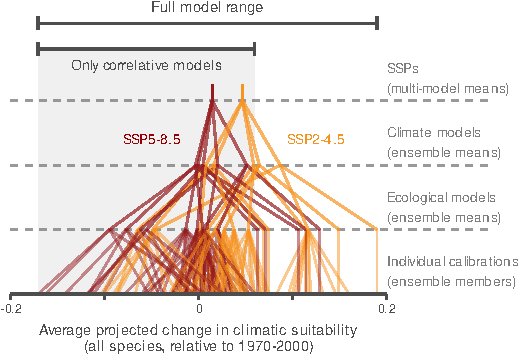
\includegraphics[width=0.75\linewidth]{figures/allspecies_cascade.pdf}
	\caption{\textbf{Considering a broad range of models provides a more comprehensive view of possible future scenarios.} This figure illustrates the average change in suitability across all species and all biomes, with the hirarchical contribution of each source of uncertainty. The top of each cascade represents the overall average change in suitability for each SSP. The level below shows the ensemble mean for each climate model (5 branches per SSP, corresponding to the 5 GCMs considered here), averaged across multiple ecological models. The next level represents the contribution of each ecological modeling approach (mechanistic, hybrid, and correlative, 3 branches per GCM). The final level displays the variations within each approach (e.g., different parameter calibrations or statistical algorithms), although for mechanistic models only a single calibration was available. This figure was inspired by the Figure 1.15 in IPCC, 2021: Chapter 1.}
	\label{fig:cascade}
\end{figure}

% [Maybe something on using existing range data leads to more pessimistic forecasts?]
%emw19May -- below when you say ' that models calibrated using current species range data consistently predict greater extinctions than models calibrated using experimental data ' do you just mean correlative vs. mechanistic? If so, I would stick with those terms. If otherwise, I would introduce what you mean as new second sentence in paragraph.
Using a comprehensive set of models allows to avoid the specific biases inherent to some modeling approaches. Our results revealed that models calibrated using current species range data consistently predict greater extinctions than models calibrated using experimental data (\Cref{fig:diffproj}). 
%Especially in Mediterranean and Atlantic ecoregions and in the western part of the Continental ecoregion (Figures 23). Overall, expert PEMs also simulated a higher increase of suitability in the transition zone between Continental and Boreal ecosystems. Fitted PEMs
Current distribution data may capture only a portion of the climatic niche of a species, underestimating the range of conditions where it could survive \citep{Chevalier2024, NoguesBravo2016}.
% do not account for the physiological processes behind species distribution
These discrepancies between models can significantly alter country-level projections, and impact national strategies derived from them. 
For example, by the end of the 21st century, beech showed an average suitability decrease of -0.19 ($\pm$0.14) across its historical distribution when considering only models entirely calibrated with current species distribution data, leading to an average loss of 30.5\% of its historical distribution (\Cref{fig:diffproj}). But this decreasing trend vanishes once a broad range of models is accounted for (-0.028 $\pm$0.17).
Relying on a narrow set of models---especially derived from the same calibration process---undermines the robustness of projections \citep{Dawson2011}, and may ultimately bias decisions towards intensive intervention strategies (e.g. introduction of species outside their native range), potentially overlooking alternative strategies.
% Multi-model ensembles have been so far mostly restricted to statistical models (Simmonds et al, 2024), but we show here that there is a strong interest in considering a broader range of models to better characterize projections uncertainty. 


% \item which implications in terms  of forest management? 
%\begin{enumerate}
%	\item on average, uncertain projections = more possibilities to act? more adaptation measures
%	\item but high uncertainties may lead to \emph{laissez-faire}
%	\item we want to avoid that, how to translate uncertainties into decision-making?\\
%	$\rightarrow$ favor forest adaptation strategies resilient to a wide range of possible future conditions.
%	\item forest managers, policy makers:\\
%	rethink the way species distribution modeling is applied to forest management\\
%\end{enumerate}

\begin{figure}
	\centering
	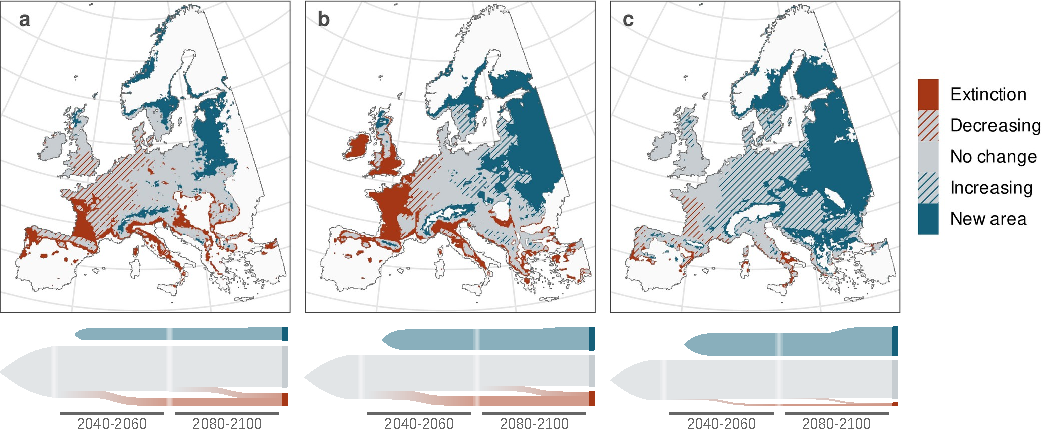
\includegraphics[width=1\linewidth]{figures/fagus_sankey.pdf}
	\caption{\textbf{Models build on current species range data project higher extinctions.} This figure illustrates the average projection of beech distribution under scenario SSP2-4.5, for each of the 3 ecological modeling approaches considered here: \textbf{(a)} correlative, \textbf{(b)} hybrid and \textbf{(c)} mechanistic models. The upper maps show the projected change in beech distribution for 2080–2100, relative to its historical distribution (1970-2000). The lower Sankey diagrams illustrate the temporal evolution of beech distribution, from its historical distributions to projected distributions for 2040–2060 and 2080–2100.}
	\label{fig:diffproj}
\end{figure}

% Isabelle: to distinguish areas with relatively consistent projections where precise actions for adaptation can be decided with larger confidence, from areas with inconsistent projections where a larger portfolio of actions should be considered considering the larger uncertainty.
% Despite large uncertainties, comparing diverse models improve prediction robustness and enable to identify areas with relatively consistent projections that differ in terms of future climate risks and levers of action to address them (\Cref{fig:manag}).

%emw19May -- consider a subheader? 
Subheader: Moving forward with management despite uncertainties 

Despite large uncertainties, comparing diverse models improve prediction robustness and enable to identify areas with relatively consistent projections where precise actions for adaptation can be decided with larger confidence (\Cref{fig:manag}).
Around the Mediterranean Basin, the models consistently predict less favorable climatic conditions for the species we considered here. In areas where most species are threatened, forest managers may thus consider introducing more drought-tolerant species. Along the Atlantic margin, the suitability of most species is also projected to decrease, except for the two Mediterranean species---pubescent and evergreen oaks--- which could replace less adapted temperate species such as beech \citep{Penuelas2003}. Mechanistic model projections are less pessimistic for deciduous oaks and beech (\Cref{fig:diffproj}), suggesting that some better-adapted populations could survive if the existing standing genetic variation is maintained and promoted by forest managers \citep{Brang2014}. Additionally, adapting management practices, such as decreasing stand density to limit competition for water, could support their long-term survival to drought events \citep{Young2023}.
Finally, boreal biomes in Scandinavian and Baltic countries are projected to get an overall increase of climatic suitability (\Cref{fig:manag}). These include Finland and Sweden, two very important forestry countries in terms of wood stock, added value, and forest-based workforce [cite].
Forests in these regions are dominated by two conifers species, Scots pine and spruce, favoured by commercial forest management. Insufficient experimental data prevented us from making mechanistic model projections for spruce, but uncertainty for Scot pine future suitability was very high. Models consistently project that temperate deciduous trees will become more competitive at the northern margin of their range (\Cref{fig:diffproj}), and the extending growing season could offer an opportunity to convert pure coniferous stands into mixed forest to increase their resilience \citep{Schauer2023}.

%emw19May --  I got confused here, as the paragraph seemed to have conflicting information (it's totally uncertain, then: here's some stuff that is consistent enough to act on) so I charged forward and wrote up what COULD be happening but you would know better than me. 
Our framework also allow to identify regions of high uncertainty, highlighting where diversification strategies are most required.
% where policies to be carefully tailored to effectively address all uncertainties
A large part of the Continental biome exhibit less clear trends (\Cref{fig:manag}), as well as mountainous regions at the transition between Mediterranean and Continental/Atlantic climates (Pyrenees, Massif Central, Balkans). A key lever of action in this region is the diversification of tree species, as well as increasing genetic diversity within populations, to mitigate the risks associated with uncertain future conditions \citep{Morin2014, Ammer2019, Pretzsch2021, Vospernik2024}. Promoting uneven-aged stands could also enhance forest stability by improving structural complexity and buffering against climate extremes \citep{Vangi2024, Zhang2024a}.

Even in these highly uncertain regions our approach still highlights some smaller zones of consistency. Models agree on a lower suitability for Scots pines (with uncertainty driven more by climatic models and scenarios, 45.7\%, than by ecological models, 30.8\%), which is a commercially very important species [cite] in several countries of Central Europe (such as Poland, Eastern Germany, Czech Republic, Belarus).
Projections also suggest that temperate deciduous species (e.g. beech, deciduous oaks) will be less affected by climate change, despite high uncertainties due to high divergence among ecological models (between 45.7 and 75.4\% of the total uncertainty). %emw19May -- end with some wrap up sentence here? I also wonder if this paragraph should be swapped with the previous one (with some edits for flow) so that you end on the highest uncertainty. 


% idea: Forest management decisions can only be made alongside the development of economic sectors for deciduous species

% Europe: 38.6% forest, and most countries have at least 30% of forest
% Germany account for 13.2% of the stock of timber in the EU's forests 
% Sweden: 12.6% - France : 11.8%, then Poland, Finland Romania, all > 8%
% => these five countries represent more than 50%
%  largest workforce: Sweden, Romania, Germany
% from my PhD discussion:
% As perfectly summarized by \citet{Dawson2011}, "\emph{the heavy reliance of conservation management and policy on a single scientific approach creates risks of policy or management failures, particularly given that the underlying assumptions of that approach are under debate}". Indeed, we have shown that the discrepancies between the different modeling approaches we considered represent a significant share of the uncertainties of future species range shifts (\Cref{fig:cascadebonus}). Researchers may omit some uncertainties because they believe communicating on them can have a negative effect on public trust \citep{Howe2019, Simmonds2024} and may prefer to deliver what they consider a clear message -- sometimes to favor the publication of their results in a competitive academic world \citep{Yao2023}. However, this is a poor strategy because it may decrease public support for science in the long term, particularly if exaggerated pessimistic projections do not ultimately occur \citep{Kreps2020}. Expressing uncertainties may indeed have constructive effects on scientists' credibility, and increase the number of people more supportive of initiatives to tackle climate change \citep{Howe2019}. Importantly, ignoring these uncertainties may also lead to poor management decisions \citep{Simmonds2024}. It could favor intensive intervention strategies (e.g. introduction of species outside their native range), while it might be possible to rather enhance the forest's genetic adaptive capacity. Quantifying and communicating uncertainties -- including by integrating different modeling approaches -- is one of the way to make ecological modeling more relevant to decision making \citep{Dietze2017, Saltelli2020}. 

\begin{figure}
	\centering
	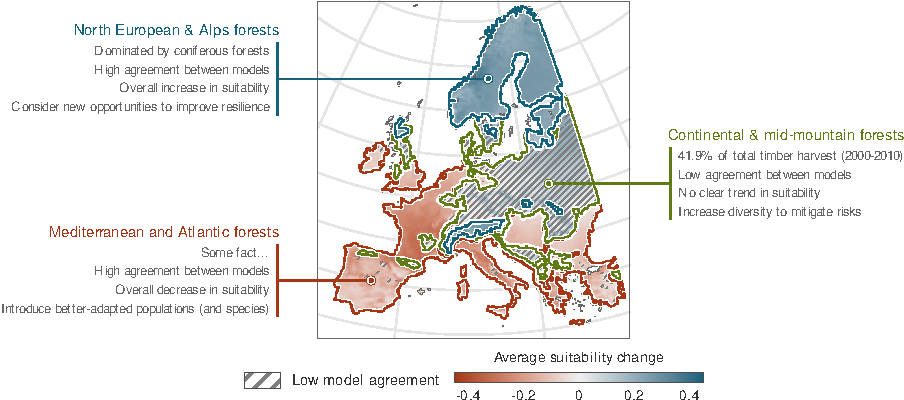
\includegraphics[width=1\linewidth]{figures/suit3-1.pdf}
	\caption{\textbf{Accounting for uncertainties supports evidence-based forest management.} Our framework allows to identify 3 areas that differ in terms of uncertainty levels, future climate risks and levers of action to address them.}
	\label{fig:manag}
\end{figure}
% conifer-dominated forestry

%emw19May -- consider a subheader? 
Subheader: Advancing on two fronts: move forward with uncertainty while aiming to reduce it through improved ecological models

% New paragraph, mentioning NA and Asia?
The implications of these results extend beyond European forests. Mechanistic models have also been developed for North America and Asia \citep{Morin2007, Fang2022}. Their projections could be systematically integrated in a comprehensive framework such as ours, alongside correlative model projections. Such continental-scale uncertainty assessment---going beyond regional analyses \citep{Iverson2016}---would provide more robust guidance for forest management. This is particularly critical in countries where forests are managed at a broader scale than in Europe--such as the United States---and where it could thus be easier to incorporate uncertainty into large-scale decision making. 

Given the rapid pace of climate change, rather than debating over which modeling approach to favor, efforts should focus on bridging diverse methodologies to generate practical insights and support evidence-based decision making. Ultimately, as scientists, we need to be transparent about projection uncertainties if we expect forest managers to acknowledge and integrate them \citep{Saltelli2020}. This is how ecological modeling can become truly relevant to decision making in the face of a changing climate.

Such an approach does not preclude continuing to improve ecological models to reduce their uncertainty. 
%emw19May -- I commented out below sentence as it's too similar to the NEXT one, but either works I think. 
% One of the key challenges for reducing projection uncertainty remains at the biological and ecological levels---even before considering the broad variations across future climate projections---highlighting that we should continue improving models. 
The large uncertainties we found clearly raise questions about the robustness of existing projections, and highlight that further advances are necessary to provide the most useful projections for managers and for policy. 
Correlative models are becoming more mechanistic by integrating experimental data \citep{Wagner2023}---yet, with some caution \citep{Chevalier2024a}. Combining deep learning with physics-based models offers a promising approach to improve climate predictions \citep{Kochkov2024}, with a lower computational cost that could facilitate a more comprehensive estimation of uncertainties. These breakthroughs are continually enhancing our ability to make robust ecological and climatological forecasts, and could in turn reveal new innovative pathways for forest management. But the need for this improvement should not prevent us from providing a better framework to identify uncertainty in projections that can guide management, such the framework we offer here.  %emw19May --  I think you can cut the first sentence I added here ('Such an approach does not preclude continuing ...') and then consider moving this paragraph FIRST in this new subsection. See if you think it works!
% there is no time for fruitless debates over which modeling approach to favor. Instead, 
% Interdisciplinary synergies will be essential to developing models that are both grounded in mechanistic understanding and statistically robust. 
% Mechanistic model improvements should go beyond mere sophistication---adding new processes and new parameters---toward robust statistical inference. Too often, mechanistic models often rely on a single immutable best-parameter set per species \citep{Harrison2021}, preventing any proper propagation of uncertainty. 


%Looking ahead: a call to action for the scientific community...
%\begin{itemize}
%\item the rapid pace of climate change leaves no time for debates over which modeling approach to favor. Instead, efforts should focus on bridging different methodologies to generate practical insights and support evidence-based decision making.
%\item take advantage of interdisciplinary synergies to build models that are not only grounded in the current mechanistic understanding of the processes but also statistically robust
%\item recent trend to refine correlative models relies on the integration of experimental data \citep{Kuo2022}
%\item mechanistic model refinement should rely not only on sophistication (i.e. adding new processes and parameters)...
%\item we need to go further into uncertainty evaluation, e.g. moving from the \emph{one-unique-parameter-set paradigm} in mechanistic models \citep{Harrison2021}, favor robust inference methods to improve uncertainty propagation
%\item us, as scientists, we need to be transparent about these uncertainties if we want forest managers to tackle them, to include them in the decision making process, i.e. if we want to make ecological modeling more relevant to decision making \citep{Saltelli2020}
%\end{itemize}

%	 substantial progress required to develop more reliable projections
%	\item proper evaluation of the transferability?
%  	\item far from l'opposisiton non constructive de differentes ecoles, hypotheses, bridge across to gain practical insights
% M, but also on a step-by-step reassessment and reformulation of the model assumptions, 
%	we have to learn from the different approach, integrate them, of fewer, but more robust models that incorporate mechanistic understanding? simple models can also be great, especially at this scale! considering more diverse data, e.g. phylogeny
% statistical models are evolving towards more mechanistic approaches, 
%	\item going further ? (parameter uncertainty is totally ignored in process-explicit models...), 
%	$\rightarrow$ , i.e; we need to build on similar framework to actually guide adaptation
%\end{enumerate}
% Quantifying and communicating uncertainties -- including by integrating different modeling approaches -- is one of the way to  \citep{Dietze2017, Saltelli2020}. 

\subsection*{Methods}

\subsubsection*{Species distribution models}

We sought to encompass a broad diversity of species distribution models by including three different approaches: correlative models, mechanistic models and hybrid models (i.e. mechastic models calibrated like correlative models\citep{VanderMeersch2023}).

For the correlative approach, we selected four well-established models\citep{Valavi2022}: GLM with lasso regularization, GAM, BRT, and down-sampled Random Forest. For the mechanistic approach, we used the process-based model PHENOFIT. The model has been validated for several North American and European species, either in historical or Holocene climatic conditions \citep{Morin2007, Saltre2013, Duputie2015, Gauzere2020, VanderMeersch2024}. For the hybrid approach, we calibrated PHENOFIT using the same species occurrence data as correlative models\citep{VanderMeersch2023}. We optimized the parameters of the model using the covariance matrix adaptation evolution strategy\citep{Hansen2001}.

\subsubsection*{Cliamte projections}

Future simulations were run with the last Coupled Model Intercomparison Project Phase 6 (CMIP6) climate  projections, for 5 global climate models (GCMs) and 2 shared socio-economic pathways (SSPs). 
We used model projections that were downscaled to a 0.1° resolution with a statistical trend-preserving method (the cumulative distribution function transform), using the ERA5-Land reanalysis as a reference observational dataset between 1981 and 2010 \citep{Noel2022}. The five GCMs were GFDL-ESM4 \citep{Dunne2020}, IPSL-CM6A-LR \citep{Lurton2020}, MPI-ESM1-2-HR \citep{Mueller2018}, MRI-ESM2-0 \citep{Yukimoto2019} and UKESM1-0-LL \citep{Sellar2020}. They are considered as good representatives of the full CMIP6 ensemble \citep{Noel2022}. 

\subsubsection*{Uncertainty partitioning}

Our approach was inspired by the partitioning of uncertainties in climate projections initially developed by Hawkins and Sutton \citep{Hawkins2009, Hawkins2011}, which was subsequently enhanced with additional methodologies \citep{Yip2011, Lafferty2023}. Rather than using a simple variance decomposition approach, we perform an ANOVA-based variance decomposition to also estimate the importance of the two-way interaction effects. All analyses were performed in R \citep{RCT2024}.

Across all species, we partitioned three sources of uncertainty: the climate projection uncertainty related to the different GCMs, SSPs, and their interaction, the species distribution modeling uncertainty related to the differents SDMs. We also considered the interactions between SDMs and climate projections (GCMs and SSPs). For each year, the suitability of a cell was considered as a 21-year moving average suitability (e.g. 2040-2060 for the year 2050). We then computed the difference of suitability with the historical suitability (c1970-2000). For each GCM and each SSP, when multiple SDM projections were simulated within the same SDM approach (e.g. multiple algorithms for correlative approach), we kept one ensemble per approach. For each year $t$, we then applied a linear ANOVA to calculate the sums of squares attributable to each uncertainty source:
$$
{SS}_{tot} = {SS}_{GCM} + {SS}_{SSP} + {SS}_{GCM:SSP} + {SS}_{SDM} + {SS}_{SDM:GCM} + {SS}_{SDM:SSP} + {SS}_{residuals}
$$

We then computed 90\% uncertainty ranges additively and symmetrically around the mean projection (across all GCMs, SSPs, SDMs), e.g. for SDM uncertainty: $\pm1.645*\sigma*\frac{{SS}_{SDM}}{{SS}_{tot}}$.


\clearpage

\bibliography{phd_bibliography}

\end{document}
